\documentclass[12pt]{article}

%%%%%%%%%%%%%%%%%%%%%%%%%%%%%%%%%%%%%%%%%%%%%%%%%%%%%%%%%%%%%%%%%%%%%%%%%%%%%%%%
%                           Package preset for homework
%%%%%%%%%%%%%%%%%%%%%%%%%%%%%%%%%%%%%%%%%%%%%%%%%%%%%%%%%%%%%%%%%%%%%%%%%%%%%%%%
% Miscellaneous
\usepackage[margin=1in]{geometry}
\usepackage[utf8]{inputenc}
\usepackage{indentfirst}
\usepackage{blindtext}
\usepackage{graphicx}
\usepackage{xr-hyper}
\usepackage{hyperref}
\usepackage{enumitem}
\usepackage{color}
\usepackage{float}
% Math
\usepackage{latexsym}
\usepackage{amsfonts}
\usepackage{amssymb}
\usepackage{amsmath}
\usepackage{commath}
\usepackage{amsthm}
\usepackage{bbold}
\usepackage{bm}
% Physics
\usepackage{physics}
\usepackage{siunitx}
% Code typesetting
\usepackage{listings}
% Citation
\usepackage[authoryear]{natbib}
\usepackage{appendix}
\usepackage[capitalize]{cleveref}
% Title & name
\title{Homework}
\author{Tien Vo}
\date{\today}


%%%%%%%%%%%%%%%%%%%%%%%%%%%%%%%%%%%%%%%%%%%%%%%%%%%%%%%%%%%%%%%%%%%%%%%%%%%%%%%%
%                   User-defined commands and environments
%%%%%%%%%%%%%%%%%%%%%%%%%%%%%%%%%%%%%%%%%%%%%%%%%%%%%%%%%%%%%%%%%%%%%%%%%%%%%%%%
%%% Misc
\sisetup{load-configurations=abbreviations}
\newcommand{\due}[1]{\date{Due: #1}}
\newcommand{\hint}{\textit{Hint}}
\let\oldt\t
\renewcommand{\t}[1]{\text{#1}}

%%% Bold sets & abbrv
\newcommand{\N}{\mathbb{N}}
\newcommand{\Z}{\mathbb{Z}}
\newcommand{\R}{\mathbb{R}}
\newcommand{\Q}{\mathbb{Q}}
\let\oldP\P
\renewcommand{\P}{\mathbb{P}}
\newcommand{\LL}{\mathcal{L}}
\newcommand{\FF}{\mathcal{F}}
\newcommand{\HH}{\mathcal{H}}
\newcommand{\NN}{\mathcal{N}}
\newcommand{\ZZ}{\mathcal{Z}}
\newcommand{\RN}[1]{\textup{\uppercase\expandafter{\romannumeral#1}}}
\newcommand{\ua}{\uparrow}
\newcommand{\da}{\downarrow}

%%% Unit vectors
\newcommand{\xhat}{\vb{\hat{x}}}
\newcommand{\yhat}{\vb{\hat{y}}}
\newcommand{\zhat}{\vb{\hat{z}}}
\newcommand{\nhat}{\vb{\hat{n}}}
\newcommand{\rhat}{\vb{\hat{r}}}
\newcommand{\phihat}{\bm{\hat{\phi}}}
\newcommand{\thetahat}{\bm{\hat{\theta}}}

%%% Other math stuff
\providecommand{\units}[1]{\,\ensuremath{\mathrm{#1}}\xspace}
% Set new style for problem
\newtheoremstyle{problemstyle}  % <name>
        {10pt}                   % <space above>
        {10pt}                   % <space below>
        {\normalfont}           % <body font>
        {}                      % <indent amount}
        {\bfseries\itshape}     % <theorem head font>
        {\normalfont\bfseries:} % <punctuation after theorem head>
        {.5em}                  % <space after theorem head>
        {}                      % <theorem head spec (can be left empty, 
                                % meaning `normal')>

% Set problem environment
\theoremstyle{problemstyle}
\newtheorem{problemenv}{Problem}[section]
\newenvironment{problem}[1]{%
  \renewcommand\theproblemenv{#1}%
  \problemenv
}{\endproblemenv}
% Set lemma environment
\newenvironment{lemma}[2][Lemma]{\begin{trivlist}
\item[\hskip \labelsep {\bfseries #1}\hskip \labelsep {\bfseries #2.}]}{\end{trivlist}}
% Set solution environment
\newenvironment{solution}{
    \begin{proof}[Solution]$ $\par\nobreak\ignorespaces
}{\end{proof}}
\numberwithin{equation}{problemenv}

%%% Page format
\setlength{\parindent}{0.5cm}
\setlength{\oddsidemargin}{0in}
\setlength{\textwidth}{6.5in}
\setlength{\textheight}{8.8in}
\setlength{\topmargin}{0in}
\setlength{\headheight}{18pt}

%%% Code environments
\definecolor{dkgreen}{rgb}{0,0.6,0}
\definecolor{gray}{rgb}{0.5,0.5,0.5}
\definecolor{mauve}{rgb}{0.58,0,0.82}
\lstset{frame=tb,
  language=Python,
  aboveskip=3mm,
  belowskip=3mm,
  showstringspaces=false,
  columns=flexible,
  basicstyle={\small\ttfamily},
  numbers=none,
  numberstyle=\tiny\color{gray},
  keywordstyle=\color{blue},
  commentstyle=\color{dkgreen},
  stringstyle=\color{mauve},
  breaklines=true,
  breakatwhitespace=true,
  tabsize=4
}
\lstset{
  language=Mathematica,
  numbers=left,
  numberstyle=\tiny\color{gray},
  numbersep=5pt,
  breaklines=true,
  captionpos={t},
  frame={lines},
  rulecolor=\color{black},
  framerule=0.5pt,
  columns=flexible,
  tabsize=2
}


\title{Homework 2: Phys 7310 (Fall 2021)}

\begin{document}


\maketitle

%%%%%%%%%%%%%%%%%%%%%%%%%%%%%%%%%%%%%%%%%%%%%%%%%%%%%%%%%%%%%%%%%%%%%%%%%%%%%%%%
\begin{problem}{2.1}[Image charge for a plane conductor]

A point charge $q$ is brought to a position a distance $d$ away from an infinite
plane conductor held at zero potential. Using the method of images, find:

(a) the surface-charge density induced on the plane, and plot it;

(b) the force between the plane and the charge by using Coulomb's law for the
force between the charge and its image;

(c) the total force acting on the plane by integrating $\sigma^2/2\epsilon_0$,
over the whole plane;

(d) the work necessary to remove the charge $q$ from its position to infinity;

(e) the potential energy between the charge $q$ and its image [compare the
answer to part (d) and discuss].

(f) Find the answer to part (d) in electron volts for an electron originally one
angstrom from the surface.

\begin{solution}

(a) Put an image charge $q'$ at $z=-d$. The total potential is
\begin{equation}
    \Phi=k\qty[
        \frac{q}{\sqrt{x^2+y^2+(z-d)^2}}
        +\frac{q'}{\sqrt{x^2+y^2+(z+d)^2}}
    ] 
\end{equation}
At $z=0$, $\Phi=0$ only if $q'=-q$. Thus,
\begin{equation}
    \Phi=\frac{q}{4\pi\epsilon_0}\qty[
    \frac{1}{\sqrt{x^2+y^2+(z-d)^2}}-\frac1{\sqrt{x^2+y^2+(z+d)^2}}
    ] 
\end{equation}
Then we can calculate
\begin{align}
    \grad\Phi
    &=-kq\Bigg\{
        \qty(x\xhat+y\yhat)
        \qty[
            \frac1{\qty(x^2+y^2+(z-d)^2)^{3/2}}
            -\frac1{\qty(x^2+y^2+(z+d)^2)^{3/2}}
        ]\notag\\
    &\qquad+\qty[
        \frac{z-d}{\qty(x^2+y^2+(z-d)^2)^{3/2}}
        -\frac{z+d}{\qty(x^2+y^2+(z+d)^2)^{3/2}}
    ]\zhat
    \Bigg\}
\end{align}
So the surface charge density is
\begin{equation}\label{p1a:sigma}
    \sigma=-\epsilon_0\eval{\grad\Phi}_{z=0}
    =-\frac{qd}{2\pi}\qty(x^2+y^2+d^2)^{-3/2}
\end{equation}
$\sigma$ is symmetric over the perpendicular plane. Thus, we need only plot a
cross section at $y=0$
\begin{center}
    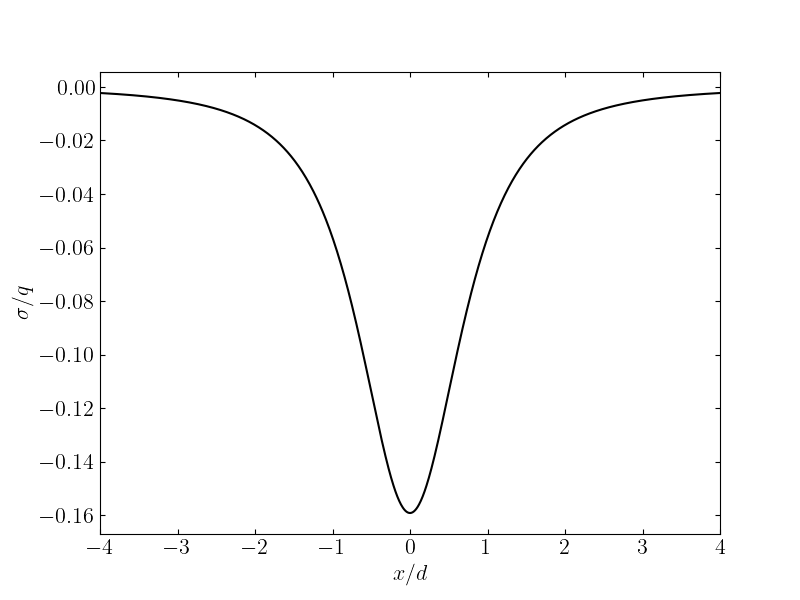
\includegraphics[width=0.8\textwidth]{p1a.png} 
\end{center}

(b) Since the distance between the two charges is $2d$, by Coulomb's law, the
force acted on the charge $q$ at $z=d$ by the charge $q'=-q$ at $z=-d$ is
\begin{equation}
    \vb{F}=-\frac1{4\pi\epsilon_0}\frac{q^2}{4d^2}\zhat 
\end{equation}

(c) From \eqref{p1a:sigma}, we can integrate
\begin{align}
    F&=\int_{\R^2}\frac{\sigma^2}{2\epsilon_0}da\notag\\
     &=\frac{q^2d^2}{8\pi^2\epsilon_0}\int_0^\infty\int_0^{2\pi}
     \frac{rdrd\theta}{(r^2+d^2)^3}\tag{$r^2=x^2+y^2$}\\
     &=\frac{q^2d^2}{4\pi\epsilon_0}\int_{d^2}^\infty\frac{du}{2u^3}
        \tag{$u=r^2+d^2$}\\
     &=\frac1{4\pi\epsilon_0}\frac{q^2}{4d^2}
\end{align}
This is the same magnitude as that in part (b).

(d) Now, from Coulomb's law, the force acted on a charge $q$ at some arbitrary 
position $z$ by the charge $q'=-q$ at $z=-d$ is
\begin{equation}
    \vb{F}=-\frac{1}{4\pi\epsilon_0}\frac{q^2}{(z+d)^2}\zhat 
\end{equation}
Then the work to move $q$ from $d$ to $\infty$ is, by definition,
\begin{align}
    W=-\int\vb{F}\vdot d\vb{l}
    =\frac{q^2}{4\pi\epsilon_0}\int_{d}^\infty\frac{dz}{(z+d)^2}
    =\frac{1}{4\pi\epsilon_0}\frac{q^2}{2d}
\end{align}
\end{solution}

(e) The potential at $z=d$ due to the charge $q'$ placed at $z=-d$ is
\begin{equation}
    \Phi(z=d)=-\frac{1}{4\pi\epsilon_0}\frac{q}{2d}
\end{equation}
Thus, the potential energy is $U=q\Phi(z=d)=-q^2/8\pi\epsilon_0d$. This is
consistent with part (d), since to remove this charge, we need to provide a work
$W=-U$ to remove the charge from the potential well.

(f) With $q=e$ and $d=1$\,\si{\angstrom}, $U=-7.2$\,\si{eV}.

\end{problem}

%%%%%%%%%%%%%%%%%%%%%%%%%%%%%%%%%%%%%%%%%%%%%%%%%%%%%%%%%%%%%%%%%%%%%%%%%%%%%%%%

\begin{problem}{2.2}[Energy in electric fields]

Starting with an expression for potential energy of a configuration of point
charges (Jackson (1.50) or (1.51)), we derived an alternate expression for the
same thing in terms of the square of the electric field generated by the charges
(Jackson (1.54)). However, along the way of the derivation we ``forgot'' the
restriction to remove the interaction of a charge with itself (``self-energy
terms''). Here we explore this.

(a) Below (1.51) is the statement to omit $i=j$ terms, so this expression for a
\textit{single} point charge is zero. Now set up the integral for formula (1.54)
for the electric field of a single point charge $q$. Show that this self-energy
integral is independent of the location of the point charge, but also that it is
infinite.

(b) Now consider two point charges $q_1$ and $q_2$; Jackson gives their electric
fieldin the unnamed equation on the top of page 42. Following Jackson in
equations (1.56-1.58), show that the energy (1.54) in this electric field is
equal to two (infinite) self-energies plus an interaction term, and show that
the interaction term takes the form you'd expect from equation (1.50). To
evaluate the integral in (1.58), show the fact Jackson gives under (1.58) is
true, and show that this fact plus our familiar expression
$\laplacian\qty(1/\abs{\vb{x}-\vb{y}})=-4\pi\delta^3(\vb{x}-\vb{y})$ also
implies that
\begin{equation}
    \div{\frac{\vb{x}-\vb{y}}{\abs{\vb{x}-\vb{y}}^3}}
    =4\pi\delta^3(\vb{x}-\vb{y}) 
\end{equation}
Thus the electric field expression for the energy of an electrostatic
configuration (1.54) is the same as (1.51) up to the self-energy terms of the
point charges. Fortunately, these self-energies are independent of position and
therefore constant! Unfortunately they are infinite, but you can't have
everything.

\begin{solution}

(a) The electric field in a coordinate where the point charge $q$ is at the 
origin is
\begin{equation}
    \vb{E}=\frac1{4\pi\epsilon_0}\frac{q}{r^2}\rhat
\end{equation}
Then the self-energy is
\begin{equation}\label{p2a:W}
    W=\frac{\epsilon_0}{2}\int_{\R^3}\abs{E}^2
    =\frac{q^2}{32\pi^2\epsilon_0}\int_{\R^3}\frac1{r^4}
    \sim\int d\Omega\int_0^\infty\frac{dr}{r^2}
    \sim\eval{-\frac1r}_0^\infty
    =\lim_{r\to0}\frac1r
\end{equation}
where $\int d\Omega=4\pi$ is the solid angle. $W\to\infty$ as $r\to0$. Note that
this is irrespective of the location of the charge, since we can always shift
into the frame where it is at the origin and evaluate the energy as in 
\eqref{p2a:W}.

(b) Given the electric field (1.56, Jackson), we can calculate
\begin{align}
    \abs{\vb{E}}^2
    &=\frac1{16\pi^2\epsilon_0^2}
        \qty[
            \frac{q_1^2\abs{\vb{x}-\vb{x}_1}^2}{\abs{\vb{x}-\vb{x}_1}^6}
            +\frac{q_2^2\abs{\vb{x}-\vb{x}_2}^2}{\abs{\vb{x}-\vb{x}_2}^6}
            +2\frac{q_1q_2\qty(\vb{x}-\vb{x}_1)\vdot\qty(\vb{x}-\vb{x}_2)}
                {\abs{\vb{x}-\vb{x}_1}^3\abs{\vb{x}-\vb{x}_2}^3}
        ]\notag\\
    &=\frac1{16\pi^2\epsilon_0^2}
        \qty[
            \frac{q_1^2}{\abs{\vb{x}-\vb{x}_1}^4}
            +\frac{q_2^2}{\abs{\vb{x}-\vb{x}_2}^4}
            +2\frac{q_1q_2\qty(\vb{x}-\vb{x}_1)\vdot\qty(\vb{x}-\vb{x}_2)}
                {\abs{\vb{x}-\vb{x}_1}^3\abs{\vb{x}-\vb{x}_2}^3}
        ]
\end{align}
It then follows from $w=\epsilon_0\abs{\vb{E}}^2/2$ that
\begin{equation}
    32\pi^2\epsilon_0w=\qty[
            \frac{q_1^2}{\abs{\vb{x}-\vb{x}_1}^4}
            +\frac{q_2^2}{\abs{\vb{x}-\vb{x}_2}^4}
            +2\frac{q_1q_2\qty(\vb{x}-\vb{x}_1)\vdot\qty(\vb{x}-\vb{x}_2)}
                {\abs{\vb{x}-\vb{x}_1}^3\abs{\vb{x}-\vb{x}_2}^3}
        ]
\end{equation}
The first two terms are self-energy. Now, we show that the last term is an
interaction term, similar to the form of (1.51, Jackson), by integrating
\begin{equation}
    W_{\text{int}}
    =\frac{q_1q_2}{16\pi^2\epsilon_0}\int_{\R^3}
        \frac{\qty(\vb{x}-\vb{x}_1)\vdot\qty(\vb{x}-\vb{x}_2)}
        {\abs{\vb{x}-\vb{x}_1}^3\abs{\vb{x}-\vb{x}_2}^3}d\vb{x}
\end{equation}
Letting $\bm\rho=(\vb{x}-\vb{x}_1)/\abs{\vb{x}_1-\vb{x}_2}$ and
$\vb{n}=(\vb{x}_1-\vb{x}_2)/\abs{\vb{x}_1-\vb{x}_2}$, it follows that
\begin{equation}
    \bm\rho+\vb{n}=\frac{\vb{x}-\vb{x}_1+\vb{x}_1-\vb{x}_2}{\abs{\vb{x}_1-\vb{x}_2}}=\frac{\vb{x}-\vb{x}_2}{\abs{\vb{x}_1-\vb{x}_2}} 
\end{equation}
Also, since $\rho_x\abs{\vb{x}_1-\vb{x}_2}=x-x_{1,x}$ where $x_{1,x}$ is the
$x$ component of $\vb{x}_1$, we can write $d\rho_x\abs{\vb{x}_1-\vb{x}_2}=dx$. 
More generally,
\begin{equation}
    d\bm\rho\abs{\vb{x}_1-\vb{x}_2}^3=
    \qty(d\rho_x\abs{\vb{x}_1-\vb{x}_2})
    \qty(d\rho_y\abs{\vb{x}_1-\vb{x}_2})
    \qty(d\rho_y\abs{\vb{x}_1-\vb{x}_2})
    =dxdydz=d\vb{x}
\end{equation}
Then we can write
\begin{align}
    \frac1{\abs{\vb{x}_1-\vb{x}_2}}\int_{\R^3} 
    \frac{\bm\rho\vdot(\bm\rho+\vb{n})}{\abs{\bm\rho}^3\abs{\bm\rho+\vb{n}}^3} d\bm\rho
    &=\frac1{\abs{\vb{x}_1-\vb{x}_2}^4}\int_{\R^3} 
    \frac{\qty(\vb{x}-\vb{x}_1)\vdot\qty(\vb{x}-\vb{x}_2)/\abs{\vb{x}_1-\vb{x}_2}^2}
    {\abs{\vb{x}-\vb{x}_1}^3\abs{\vb{x}-\vb{x}_2}^3/\abs{\vb{x}_1-\vb{x}_2}^6}d\vb{x}\notag\\
    &=\int_{\R^3}
        \frac{\qty(\vb{x}-\vb{x}_1)\vdot\qty(\vb{x}-\vb{x}_2)}{\abs{\vb{x}-\vb{x}_1}^3\abs{\vb{x}-\vb{x}_2}^3} d\vb{x}
\end{align}
and finally,
\begin{equation}\label{p2b:wint}
    W_{\text{int}}
    =\qty[\frac1{4\pi\epsilon_0}\frac{q_1q_2}{\abs{\vb{x}_1-\vb{x}_2}}]
    \times\qty[\frac1{4\pi}\int_{\R^3}\frac{\bm\rho\vdot(\bm\rho+\vb{n})}
        {\abs{\bm\rho}^3\abs{\bm\rho+\vb{n}}^3}d\bm\rho
    ]
\end{equation}
Since the term in the first square bracket already has a form resembling (1.51,
Jackson), it remains for us to show that
\begin{equation}\label{p2b:wts}
    \int_{\R^3} \frac{\bm\rho\vdot(\bm\rho+\vb{n})}
        {\abs{\bm\rho}^3\abs{\bm\rho+\vb{n}}^3}d\bm\rho=4\pi
\end{equation}
However, first we need two lemmas
\begin{lemma}{A}
    \begin{equation}\label{lA}
        \grad_\rho\qty(\frac1{\abs{\bm\rho+\vb{n}}})=-\frac{\bm\rho+\vb{n}}{\abs{\bm\rho+\vb{n}}^3} 
    \end{equation} 
\end{lemma}
\begin{quote}
\begin{proof}
    Let $\vb{R}=\bm\rho+\vb{n}=R_x\xhat+R_y\yhat+R_z\zhat$, then it follows 
    that $\grad_\rho=\grad_R$ and
    \begin{align*}
        \grad_R\qty(\frac1R)
        =-\qty(\frac{R_x}{R^3}\xhat+\frac{R_y}{R^3}\yhat+\frac{R_z}{R^3}\zhat)
        =-\frac{\vb{R}}{R^3}
        =-\frac{\bm\rho+\vb{n}}{\abs{\bm\rho+\vb{n}}^3}
    \end{align*}
\end{proof}   
\end{quote}
\begin{lemma}{B}
    \begin{equation}\label{lB}
    \div{\qty(\frac{\vb{R}}{R^3})}=4\pi\delta^3(\vb{R}) 
\end{equation} 
\end{lemma}
\begin{quote}
\begin{proof}
    From \eqref{lA}, we can take the divergence on both sides
    \begin{equation*}
        \laplacian\qty(\frac1R)=-\div{\qty(\frac{\vb{R}}{R^3})} 
    \end{equation*}
    However, we know from (1.31, Jackson) that
    $\laplacian{\qty(1/R)}=-4\pi\delta^3(\vb{R})$. Thus, by substitution,
    \eqref{lB} must be true.
\end{proof} 
\end{quote}

Now, take a spherical volume $V$ with a boundary $S=\partial V$ of radius
$\rho$, we can write the LHS of \eqref{p2b:wts} as
\begin{align}
    \text{LHS}
    =-\int_V
    \frac{\bm\rho}{\rho^3}\vdot\grad_\rho\qty(\frac1{\abs{\bm\rho+\vb{n}}})d\bm\rho
    =-\oint_{\partial V}\frac{\bm\rho\vdot
    d\vb{a}}{\abs{\bm\rho}^3\abs{\bm\rho+\vb{n}}}
+\int_V\frac1{\abs{\bm\rho+\vb{n}}}\div{\qty(\frac{\bm\rho}{\rho^3})}d\bm\rho
\end{align}
via integration by part. Note that the first term has an integrand
evaluated at $\rho=$ const on the surface $S=\partial V$. In the case that
$V\to\R^3$, $\rho\to\infty$, and since the integrand scales as $1/\rho^3$, the
boundary integral vanishes. Applying \eqref{lB} to the second integral, we get
\begin{equation}
    \int_{\R^3} \frac{\bm\rho\vdot(\bm\rho+\vb{n})}
        {\abs{\bm\rho}^3\abs{\bm\rho+\vb{n}}^3}d\bm\rho
    =4\pi\int_{\R^3}\frac{\delta^3(\bm\rho)}{\abs{\bm\rho+\vb{n}}}d\bm\rho
    =4\pi
\end{equation}
because $\abs{\vb{n}}=1$. Then from \eqref{p2b:wint}, we can write
\begin{equation}
    W_{\text{int}}=\frac1{4\pi\epsilon_0}\frac{q_1q_2}{\abs{\vb{x}_1-\vb{x}_2}} 
\end{equation}
in the same form as an interaction potential energy.


\end{solution}
 
\end{problem}

%%%%%%%%%%%%%%%%%%%%%%%%%%%%%%%%%%%%%%%%%%%%%%%%%%%%%%%%%%%%%%%%%%%%%%%%%%%%%%%%

\begin{problem}{2.3}[Neumann Green's function]
For a general Green's function $G(\vb{x},\vb{x}')$ for Poisson's equation, the
value of the potential $\Phi(\vb{x})$ in a volume $V$ with boundary surface $S$
is related to the charge density $\rho(\vb{x})$ inside $V$ and the boundary
values for $\Phi$ and $\partial\Phi/\partial n$ on $S$, by the Jackson's 
equation (1.42). When we know the value of $\Phi$ on $S$ (Dirichlet boundary
conditions), we can choose a Dirichlet Green's function oberying
$G_D(\vb{x},\vb{x}')=0$ for $\vb{x}'$ on $S$, and then find a solution for
$\Phi(\vb{x})$ in $V$ given $\rho$ and our boundary values of $\Phi$.

When we know $\partial\Phi/\partial n$ on $S$, these are Neumann boundary
conditions. Analogously to the Dirichlet case we might think we would like to
find a Green's function $G_N(\vb{x},\vb{x}')$ obeying $\partial
G_N(\vb{x},\vb{x}')/\partial n'=0$ for $\vb{x}'$ on $S$. However, this is not
possible!

(a) Any Green's function for Poisson's equation obeys Jackson (1.39) by
definition. Show that this implies that for any Poisson Green's function,
\begin{equation}
    \oint_Sda'\frac{\partial G}{\partial n'}=-4\pi 
\end{equation}
Observe this makes it impossible for $\partial G_N(\vb{x},\vb{x}')/\partial n'$
to be zero for every $\vb{x}'$ on $S$.

(b) Since $\partial G_N/\partial n'$ cannot be zero for every $\vb{x}'$ on the
boundary, the simplest condition is for $\partial G_N/\partial n'$ to be
constant for every $\vb{x}'$ on the boundary, as in Jackson (1.45). Show that
Jackson (1.45) indeed satisfies the equation from part (a) (this is easy), and
show that this leds to the solution for $\Phi(\vb{x})$ in Jackson (1.46). Thus
knowing the Neumann boundary data $\partial\Phi/\partial n$ doesn't quite get us
$\Phi(\vb{x})$ everywhere in $V$, but it gets us the deviation from the average
value on the boundary $\Phi(\vb{x})-\expval{\Phi}_S$. (Fortunately a constant
shift in the potential drops out of physical quantities!)

\begin{solution}

    (a) Using Gauss theorem, we can integrate 
    \begin{align}
        \int_V\laplacian' Gd^3x'
        &=\int_V\grad'\vdot\qty(\grad'G)d^3x'
        =\oint_S\grad'G\vdot\nhat da'
        =\oint_S\frac{\partial G}{\partial n'}da'
    \end{align}
    where $\partial G/\partial n'=(\nhat\vdot\grad')G$ is the directional
    derivative in the normal direction $\nhat$. From (1.39, Jackson),
    $\int_V\laplacian'Gd^3x'=-4\pi\int_V\delta^3(\vb{x}-\vb{x}')d^3x'=-4\pi$.
    Thus, it follows that
    \begin{equation}\label{p3a:wts}
        \oint_S da'\frac{\partial G}{\partial n'}=-4\pi 
    \end{equation}

    (b) If $\partial G/\partial n'$ is a constant, then we can pull it out of
    the integral in \eqref{p3a:wts}
    \begin{equation}
        \frac{\partial G}{\partial n'}\oint_Sda'=\frac{\partial G}{\partial
        n'}S=-4\pi 
    \end{equation}
    where $S=\oint_Sda'$ is the surface area of the bounding surface. Thus,
    \begin{equation}
        \frac{\partial G}{\partial n'}=-\frac{4\pi}{S} 
    \end{equation}
    Now, we can write from (1.42, Jackson)
    \begin{align}
        \Phi(\vb{x})&=\frac1{4\pi\epsilon_0}\int_V\rho(\vb{x}')G(\vb{x},\vb{x}')d^3x'
        +\frac1{4\pi}\oint_SG(\vb{x},\vb{x}')\frac{\partial\Phi(\vb{x}')}{\partial
        n'}da'
        -\frac1{4\pi}\frac{\partial G}{\partial
        n'}\oint_S\Phi(\vb{x}')da'\notag\\
        &=\frac1S\oint_S\Phi(\vb{x}')da'+\frac1{4\pi\epsilon_0}\int_V\rho(x')G(\vb{x},\vb{x}')d^3x'
        +\frac1{4\pi}\oint_SG(\vb{x},\vb{x}')\frac{\partial\Phi(\vb{x}')}{\partial
        n'}da'\notag\\
        &=\expval{\Phi}_S+\frac1{4\pi\epsilon_0}\int_V\rho(x')G(\vb{x},\vb{x}')d^3x'
        +\frac1{4\pi}\oint_SG(\vb{x},\vb{x}')\frac{\partial\Phi(\vb{x}')}{\partial
        n'}da'
    \end{align}
    where $\expval{\Phi}_S=(1/S)\oint_S\Phi(\vb{x}')da'$ is the average value of
    the potential on the boundary surface.
\end{solution}

\end{problem}

%%%%%%%%%%%%%%%%%%%%%%%%%%%%%%%%%%%%%%%%%%%%%%%%%%%%%%%%%%%%%%%%%%%%%%%%%%%%%%%%

\begin{problem}{2.4}[Green's function for a plane conductor]

Consider a potential problem in the half-space defined by $z\geq 0$, with
Dirichlet boundary conditions on the plane $z=0$ (and at infinity).

(a) Write down the appropriate Green function $G(\vb{x},\vb{x}'$).

(b) If the potential on the plane $z=0$ is specified to be $\Phi=V$ inside a
circle of radius $a$ centered at the origin, and $\Phi=0$ outside that circle,
find an integral expression for the potential at the point $P$ specified in
terms of cylindrical coordinates ($\rho,\phi,z$).

(c) Show that, along the axis of the circle ($\rho=0$), the potential is given
by
\begin{equation}
    \Phi=V\qty(1-\frac{z}{\sqrt{a^2+z^2}}) 
\end{equation}

(d) Show that at large distances $(\rho^2+z^2\gg a^2$) the potential can be
expanded in a power series in $(\rho^2+z^2)^{-1}$, and that the leading terms
are
\begin{equation}\label{p4d:wts}
    \Phi=\frac{Va^2}{2}\frac{z}{\qty(\rho^2+z^2)^{3/2}}\qty[
        1-\frac{3a^2}{4(\rho^2+z^2)}+
        \frac{5(3\rho^2a^2+a^4)}{8(\rho^2+z^2)^2}+\hdots
    ]
\end{equation}
Verify that the results of part (c) and (d) are consistent with each other in
their common range of validity.

\begin{solution}

(a) Generalizing from Problem 2.1(a), a potential for a point chage placed at
$\vb{x}=(x,y,z)$ is
\begin{equation}
    \Phi(\vb{x}')=\frac{q}{4\pi\epsilon_0}
        \qty[
            \frac1{\sqrt{(x'-x)^2+(y'-y)^2+(z'-z)^2}}
            -\frac1{\sqrt{(x'-x)^2+(y'-y)^2+(z'+z)^2}}
        ]
\end{equation}
Since $\Phi=(q/4\pi\epsilon_0)G$ for a point charge, we can write the Green
function as
\begin{equation}
    G(\vb{x},\vb{x}')=\frac1{\sqrt{(x'-x)^2+(y'-y)^2+(z'-z)^2}}
            -\frac1{\sqrt{(x'-x)^2+(y'-y)^2+(z'+z)^2}}
\end{equation}

(b) Then we can differentiate
\begin{equation}\label{p4b:dG}
    \frac{\partial G}{\partial z'}
    =\frac{z-z'}{\qty[(x'-x)^2+(y'-y)^2+(z'-z)^2]^{3/2}}
    +\frac{z+z'}{\qty[(x'-x)^2+(y'-y)^2+(z'+z)^2]^{3/2}}
\end{equation}
Now, we choose a volume $V$ lying on a conductor at $z=0$
and is a hemisphere with a radius $\rho'> a$ for $z>0$ (see figure)
\begin{center}
    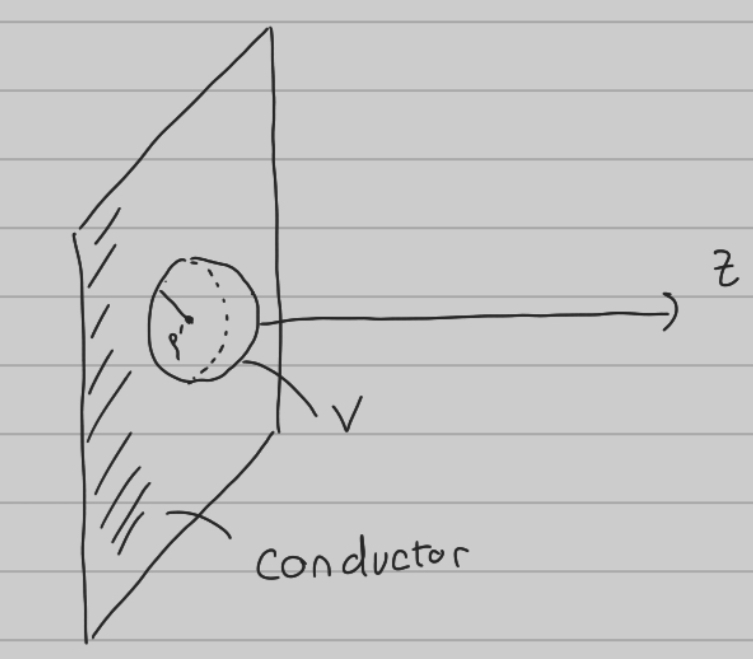
\includegraphics[width=0.5\textwidth]{hw2_p4.jpg} 
\end{center}
Then as $\rho'\to\infty$, this volume covers the half-space $z\geq0$ where all
the charge distribution is. From (1.42, Jackson),
\begin{align}
    \Phi(\vb{x})
    &=\frac1{4\pi\epsilon_0}\int_V\rho(\vb{x}')G(\vb{x},\vb{x}')d\vb{x}'
    +\frac1{4\pi}\oint_{\partial
    V}\qty[G(\vb{x},\vb{x}')\frac{\partial\Phi}{\partial
n'}-\Phi(\vb{x}')\frac{\partial G}{\partial n'}]da'\notag\\
    &=-\frac1{4\pi}\oint_{\partial V}\Phi(\vb{x}')\frac{\partial G}{\partial
    n'}da'\notag\\
    &=\frac{V}{4\pi}\oint_{\partial V}\eval{\frac{\partial G}{\partial
    z'}}_{z'=0}da'
\end{align}
where we have written $\partial G/\partial n'=-\partial G/\partial z'$ by the
choice of surface $\partial V$ (recall that $\rho'> a$). Now, as
$\rho'\to\infty$, we can write from \eqref{p4b:dG}
\begin{align}\label{p4b:Phi}
    \Phi(\vb{x})=\frac{V}{2\pi}\int_0^a\int_0^{2\pi}
    \frac{\rho'd\rho'd\phi'}{\qty[\rho^2+z^2+\rho'^2-2\rho\rho'\cos(\phi-\phi')]^{3/2}}
\end{align}
through a coordinate transformation $(x,y)=\rho(\cos\phi,\sin\phi)$ and $(x',y')=\rho'(\cos\phi',\sin\phi')$.

(c) Setting $\rho=0$, the integral \eqref{p4b:Phi} can be easily evaluated
\begin{align}
    \Phi=\frac{V}{2\pi}\int_0^a\int_0^{2\pi}\frac{\rho'd\rho'}{(\rho'^2+z^2)^{3/2}}=V\qty[1-\frac{z}{\sqrt{z^2+a^2}}] 
\end{align}
where we have used Mathematica in the last step.

(d) Factoring out $\epsilon=(\rho^2+z^2)^{-1}$, we can rewrite the integrand
$I$ in \eqref{p4b:Phi} as
\begin{align}
    I
    &=\epsilon^{3/2}\qty[1+\epsilon\qty(\rho'^2-2\rho\rho'\cos(\phi-\phi'))]^{-3/2}\notag\\
    &\approx\epsilon^{3/2}\qty[1
        -\frac32\epsilon\qty(\rho'^2-2\rho\rho'\cos(\phi-\phi'))
        +\frac{15}{8}\epsilon^2\qty(\rho'^2-2\rho\rho'\cos(\phi-\phi'))^2
        +\hdots
    ]
\end{align}
where we have expanded in order of the small parameter $\epsilon$. Integrating
each term in $I$ up to $\epsilon^3$, we get
\begin{align}\label{p4d:Phi}
    \Phi&=\frac{V}{2\pi}z\epsilon^{3/2}\int_0^a\int_0^{2\pi}\rho'd\rho'd\phi'\times\notag\\
    &\qquad\qty[1
        -\frac32\epsilon\qty(\rho'^2-2\rho\rho'\cos(\phi-\phi'))
        +\frac{15}{8}\epsilon^2\qty(\rho'^2-2\rho\rho'\cos(\phi-\phi'))^2
    ]\notag\\
    &=\frac{V}{2\pi}\frac{z}{(\rho^2+z^2)^{3/2}}\Bigg[
        \pi
        a^2-\frac32\epsilon\int_0^a\int_0^{2\pi}\rho'd\rho'\qty[\rho'^2-2\rho\rho'\cos(\phi-\phi')]\notag\\
    &\qquad+\frac{15}{8}\epsilon^2\int_0^a\int_0^{2\pi}\rho'd\rho'\qty[\rho'^4+4\rho^2\rho'^2\cos^2(\phi-\phi')-4\rho\rho'\cos(\phi-\phi')]
    \Bigg]
\end{align}
Using the fact that the $\phi$-averaged $\expval{\cos(\phi-\phi')}=0$ and
$\expval{\cos^2(\phi-\phi')}=\pi$ over a domain $[0,2\pi]$, we can simplify the
integral
\begin{align}\label{p4d:Phi_compare1}
    \Phi&=\frac{V}{2\pi}\frac{z}{(\rho^2+z^2)^{3/2}}
    \qty[\pi a^2-\frac{3\pi a^4}{4}\epsilon
    +\frac{5\pi a^2}{8}\qty(3\rho^2a^2+a^4)\epsilon^2]\notag\\
        &=\frac{Va^2}{2}\frac{z}{(\rho^2+z^2)^{3/2}}
        \qty[1-\frac{3a^2}{4}\epsilon+\frac58(3\rho^2a^2+a^4)\epsilon^2]
\end{align}
This is what we wish to shown in \eqref{p4d:wts}. For $\rho=0$, this reduces to
\begin{equation}
    \Phi=V\qty[\frac12\qty(\frac{a}{z})^2-\frac38\qty(\frac{a}{z})^4+\frac5{16}\qty(\frac{a}{z})^6] 
\end{equation}
From part (c), we can write
\begin{align}\label{p4d:Phi_compare2}
    \Phi
    &=V\qty[1-\frac{1}{\sqrt{1+(a/z)^2}}]\notag\\
    &\approx
    V\qty{1-\qty[1-\frac12\qty(\frac{a}{z})^2+\frac38\qty(\frac{a}{z})^4
    -\frac5{16}\qty(\frac{a}{z})^6+\hdots]}\notag\\
    &=V\qty[\frac12\qty(\frac{a}{z})^2-\frac38\qty(\frac{a}{z})^4
    +\frac5{16}\qty(\frac{a}{z})^6]
\end{align}
From \eqref{p4d:Phi_compare1} and \eqref{p4d:Phi_compare2}, we conclude the
answers for part (c) and (d) agree in their common range of validity.
\end{solution}
    
\end{problem}

%%%%%%%%%%%%%%%%%%%%%%%%%%%%%%%%%%%%%%%%%%%%%%%%%%%%%%%%%%%%%%%%%%%%%%%%%%%%%%%%


    
\end{document}
